\pagetopsection{ Spellweaving} \label{sec:spellweaving}

\tikz[remember picture,overlay] \node[opacity=1,inner sep=0pt] at (page cs:0.5,-0.35){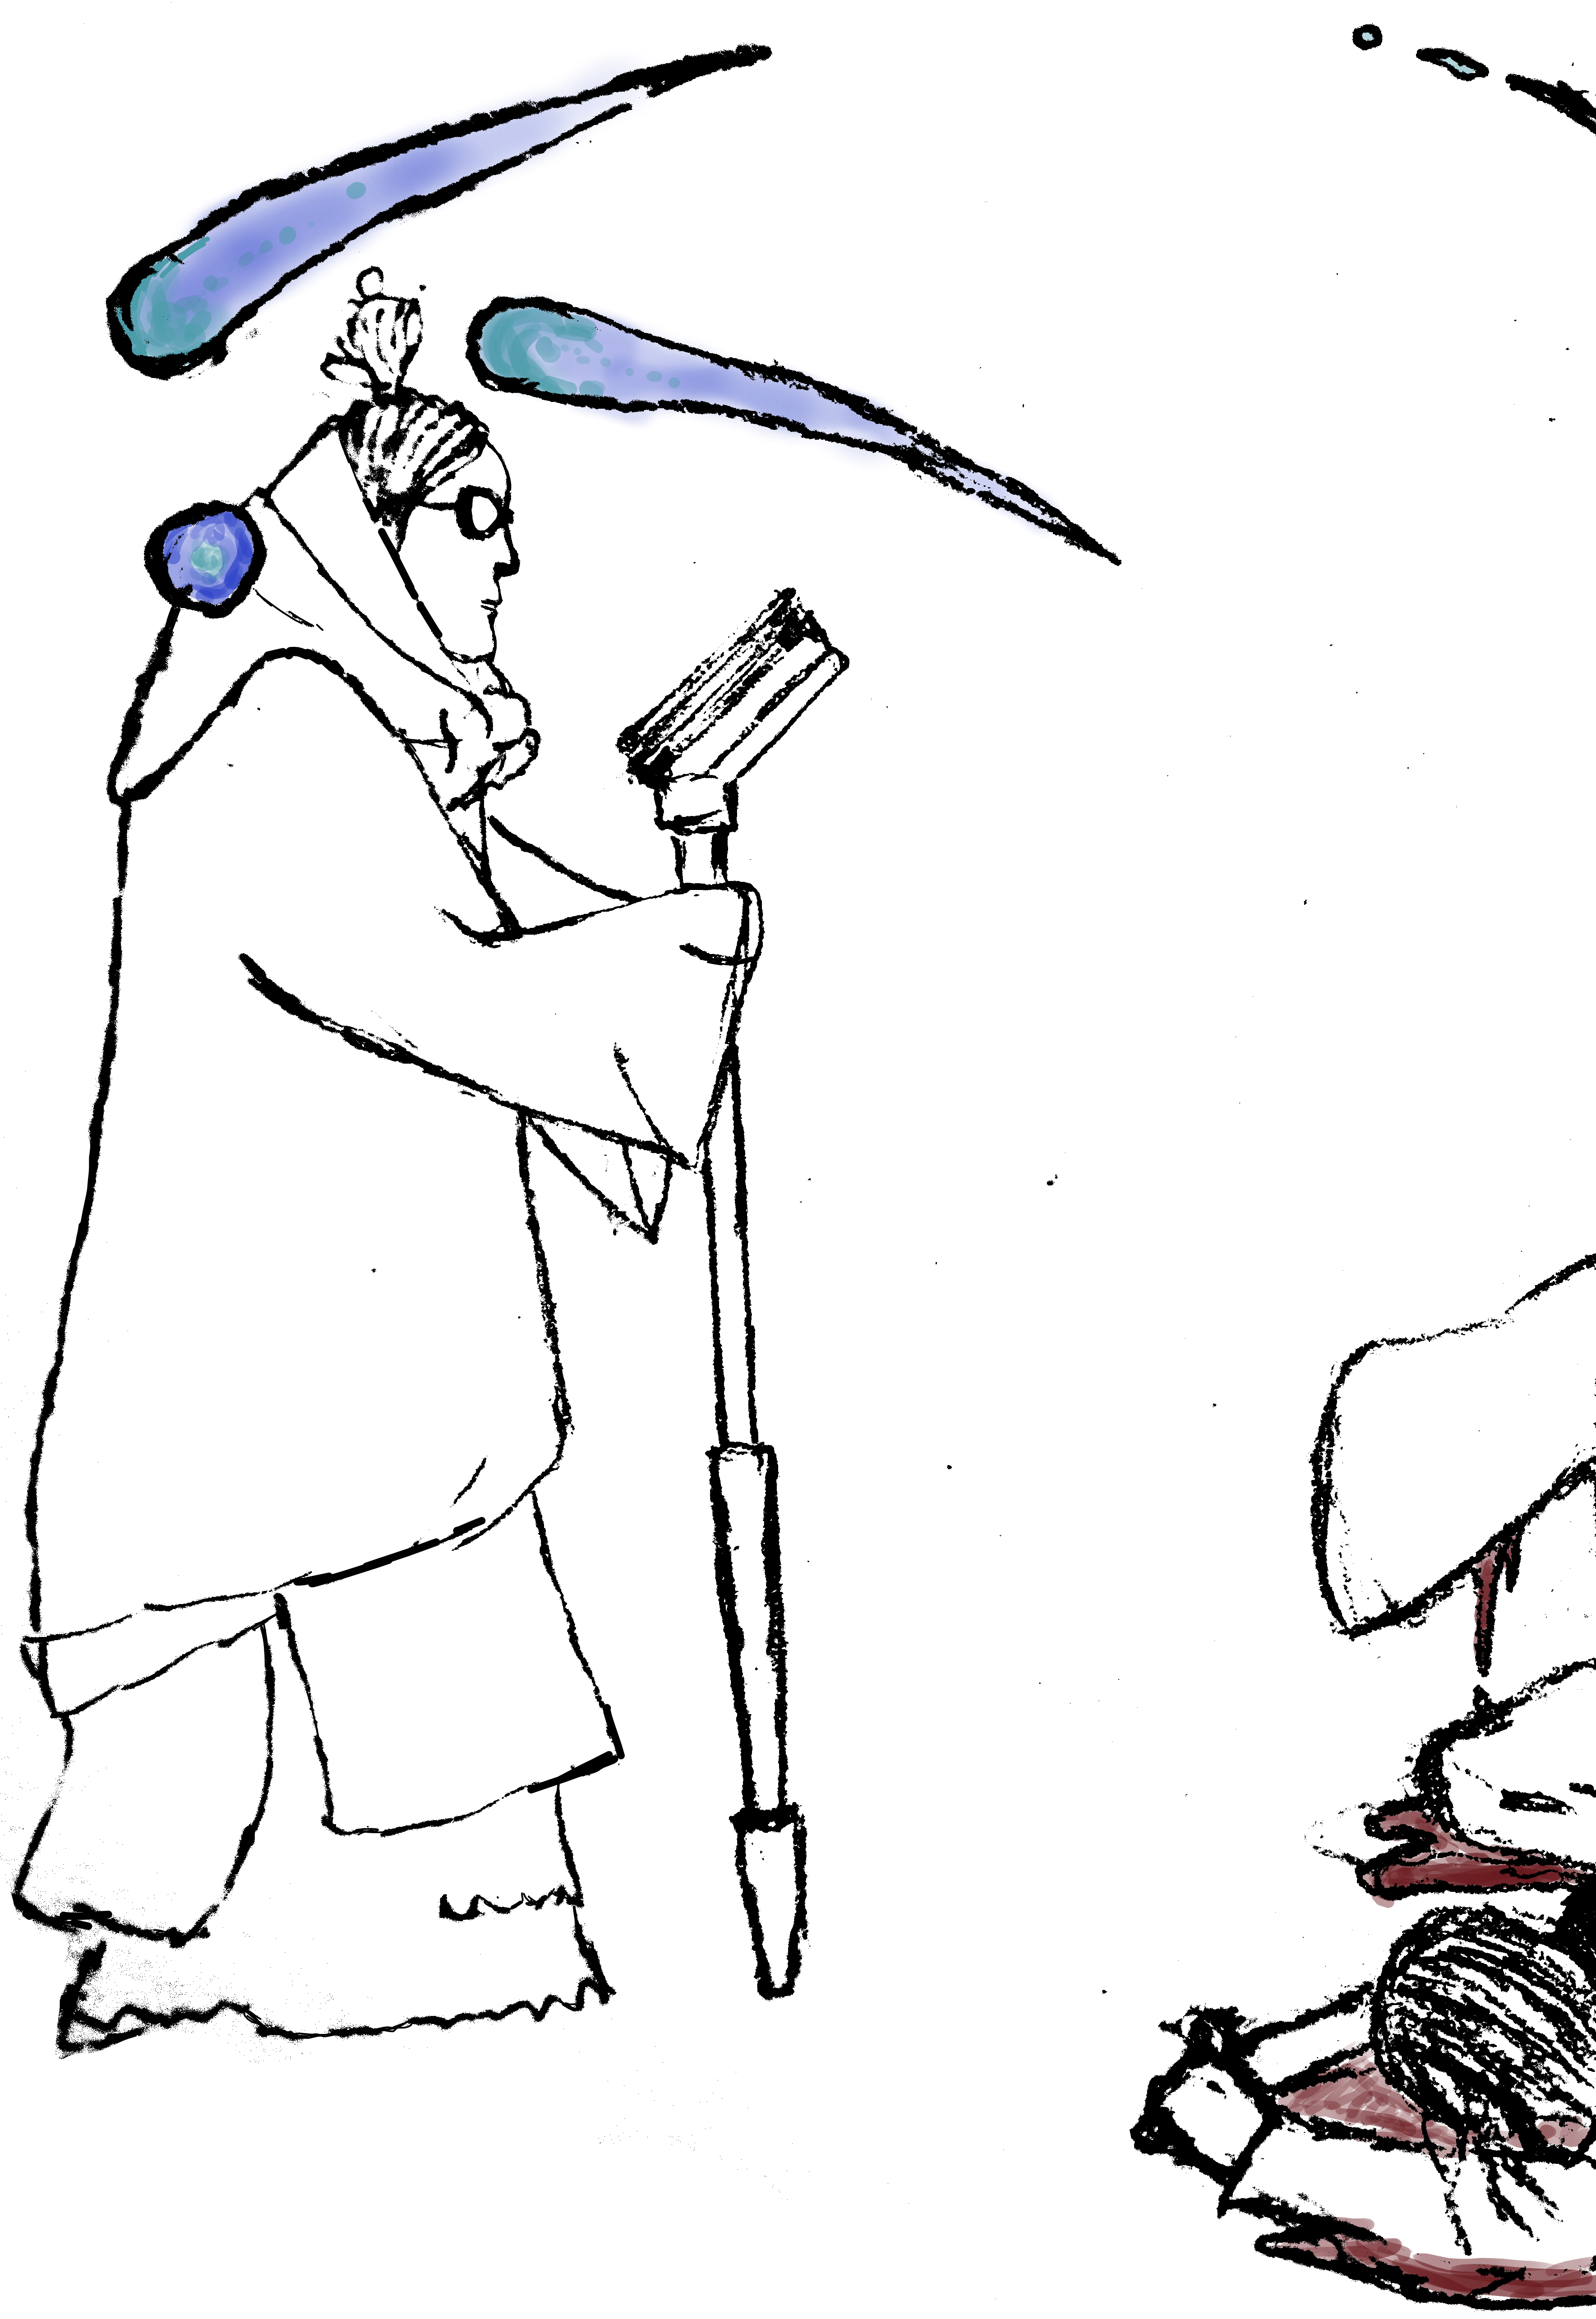
\includegraphics[width=0.5\paperwidth]{media/magic_missile_1-0.png}};

\begin{multicols*}{2}

\subsection*{Weaving a spell}

The power of a mage is represented by a \texttt{Spellweaving Pool}: a set of dice that you can use to weave spells. 

\colbox{
The spellweaving pool is described by

\begin{itemize}[nosep, leftmargin=*]
    \item Amount and kind of dice it can hold
    \item How one restores those dice
    \item What actions, if any, could change it
\end{itemize} 
}
If several effects grant you a spellweaving pool, those exist independently unless specified. Consuming \textbf{Spur} refills \texttt{3} dice from any combination of pools.

To weave a spell, a weaver rolls any number of those dice from any available pools as an Action from that set and then decides what to cast. This is a \texttt{Spellweaving roll}.
Only one spell can be cast per roll. If the spell does not state otherwise, \texttt{Smite} \texttt{Feat} is not applicable for attacks performed within them.

Each time after a spell is weaved in combat, caster needs to pass \texttt{Clarity Save} or become \texttt{Fatigued}. \textbf{No spell} can be cast until \texttt{Fatigue} is cleared.

There are many spells one can learn during their mage training, but regardless of syllabus -- all spellweavers know \textit{Detect Magic} by heart.

\newcolumn

\subsection*{Rethreading of the arcane}

When a mage rolls dice to weave a spell, in addition to casting, they can choose half, rounded down, of the remaining dice and discard the rest.
These chosen dice can be stored to cast spells later as if they are included in a roll.
They persist until spent, and count as in \texttt{Spellweaving Pool}. The amount of dice in the pool, both unused and stored, can't exceed its size.

% Several ways exist for how a person might become a mage. 
% A knight who has been taught spellweaving since childhood gets their \texttt{Spellweaving Pool} at character creation. 
% This pool is a set of \texttt{d6} dice with size equal to the value of their \texttt{Clarity}. 
% In order to restore dice, a knight must indulge their passion; this action restores \texttt{3} of them.


% \subsection*{Becoming a spellweaver}

% A knight who has been taught spellweaving gets their \texttt{Spellweaving Pool} at character creation. 
% They know any three spells from the list below in addition to \emph{Detect Magic} and one cantrip.
% \begin{itemize}[nosep, leftmargin=*]
%     \item \textbf{Dice} are all \texttt{d6}'s, and their amount is equal to the value of knights' \texttt{Clarity}.
%     \item \textbf{Restoring} the pool is done through \texttt{Overnight Rest} or indulging a \texttt{Passion}, both methods restore \texttt{3} of the missing dice.
%     \item \textbf{Improving} this pool is challenging; the limit of what could be thought is reached.
% \end{itemize}

\end{multicols*}
